\chapter{Implementation, Result, and Analysis}
\section{Overview of the approach}
Before training, we have reviewed what the chosen network requires as input.
Since we are training using synthetic dataset that would imitate our target
scenarios, we focused on generating diverse and representative samples.
\section{Dataset Preparation \& Preprocessing}
The network expects:
\begin{itemize}
    \item \textbf{Two images:} the reference image, and the target image. Stored as numpy arrays.
    \item \textbf{Two sets of keypoints:}
          \begin{itemize}
              \item \textbf{Reference keypoints:} An array of keypoint coordinates found in the reference
                    image. It has a shape of $(N, 2)$, where N is the number of keypoints, and the coordinates are (x, y).
              \item \textbf{Target keypoints:} An array of keypoint coordinates found in the target image that correspond to the reference keypoints. It has the same shape $(N, 2)$.
          \end{itemize}
    \item \textbf{Matches:} An array of shape $(N, 2)$ that stores the indices of the matching keypoints. For example, $[i, j]$ means that the i-th keypoint in the reference keypoints matches the j-th keypoint in the target keypoints.
    \item \textbf{Homography Matrix: } A 3 by 3 matrix that relates the reference icon to the target one. It is used to transform points from the reference to the target image, and vice versa.
    \item \textbf{Two binary masks:} Binary masks of the target image that indicates the region where the pixel exists. This is useful to separate the foreground from the background.
\end{itemize}
These elements would be stored as a zipped numpy file (.npz) to be later accessed during training and evaluation, and stored in a folder structure that mirrors the dataset organization.
\subsection{Data Synthesis}
\subsubsection{General Approach}
To create a diverse and representative dataset, we employed data synthesis
techniques that will allow us to experiment with various scenarios. Our general
idea consists of cropping a region of interest from the selected gaming frames,
this will help us simulate different viewpoints where the targeted 2D template
may appear.
\begin{figure}[H]
    \centering
    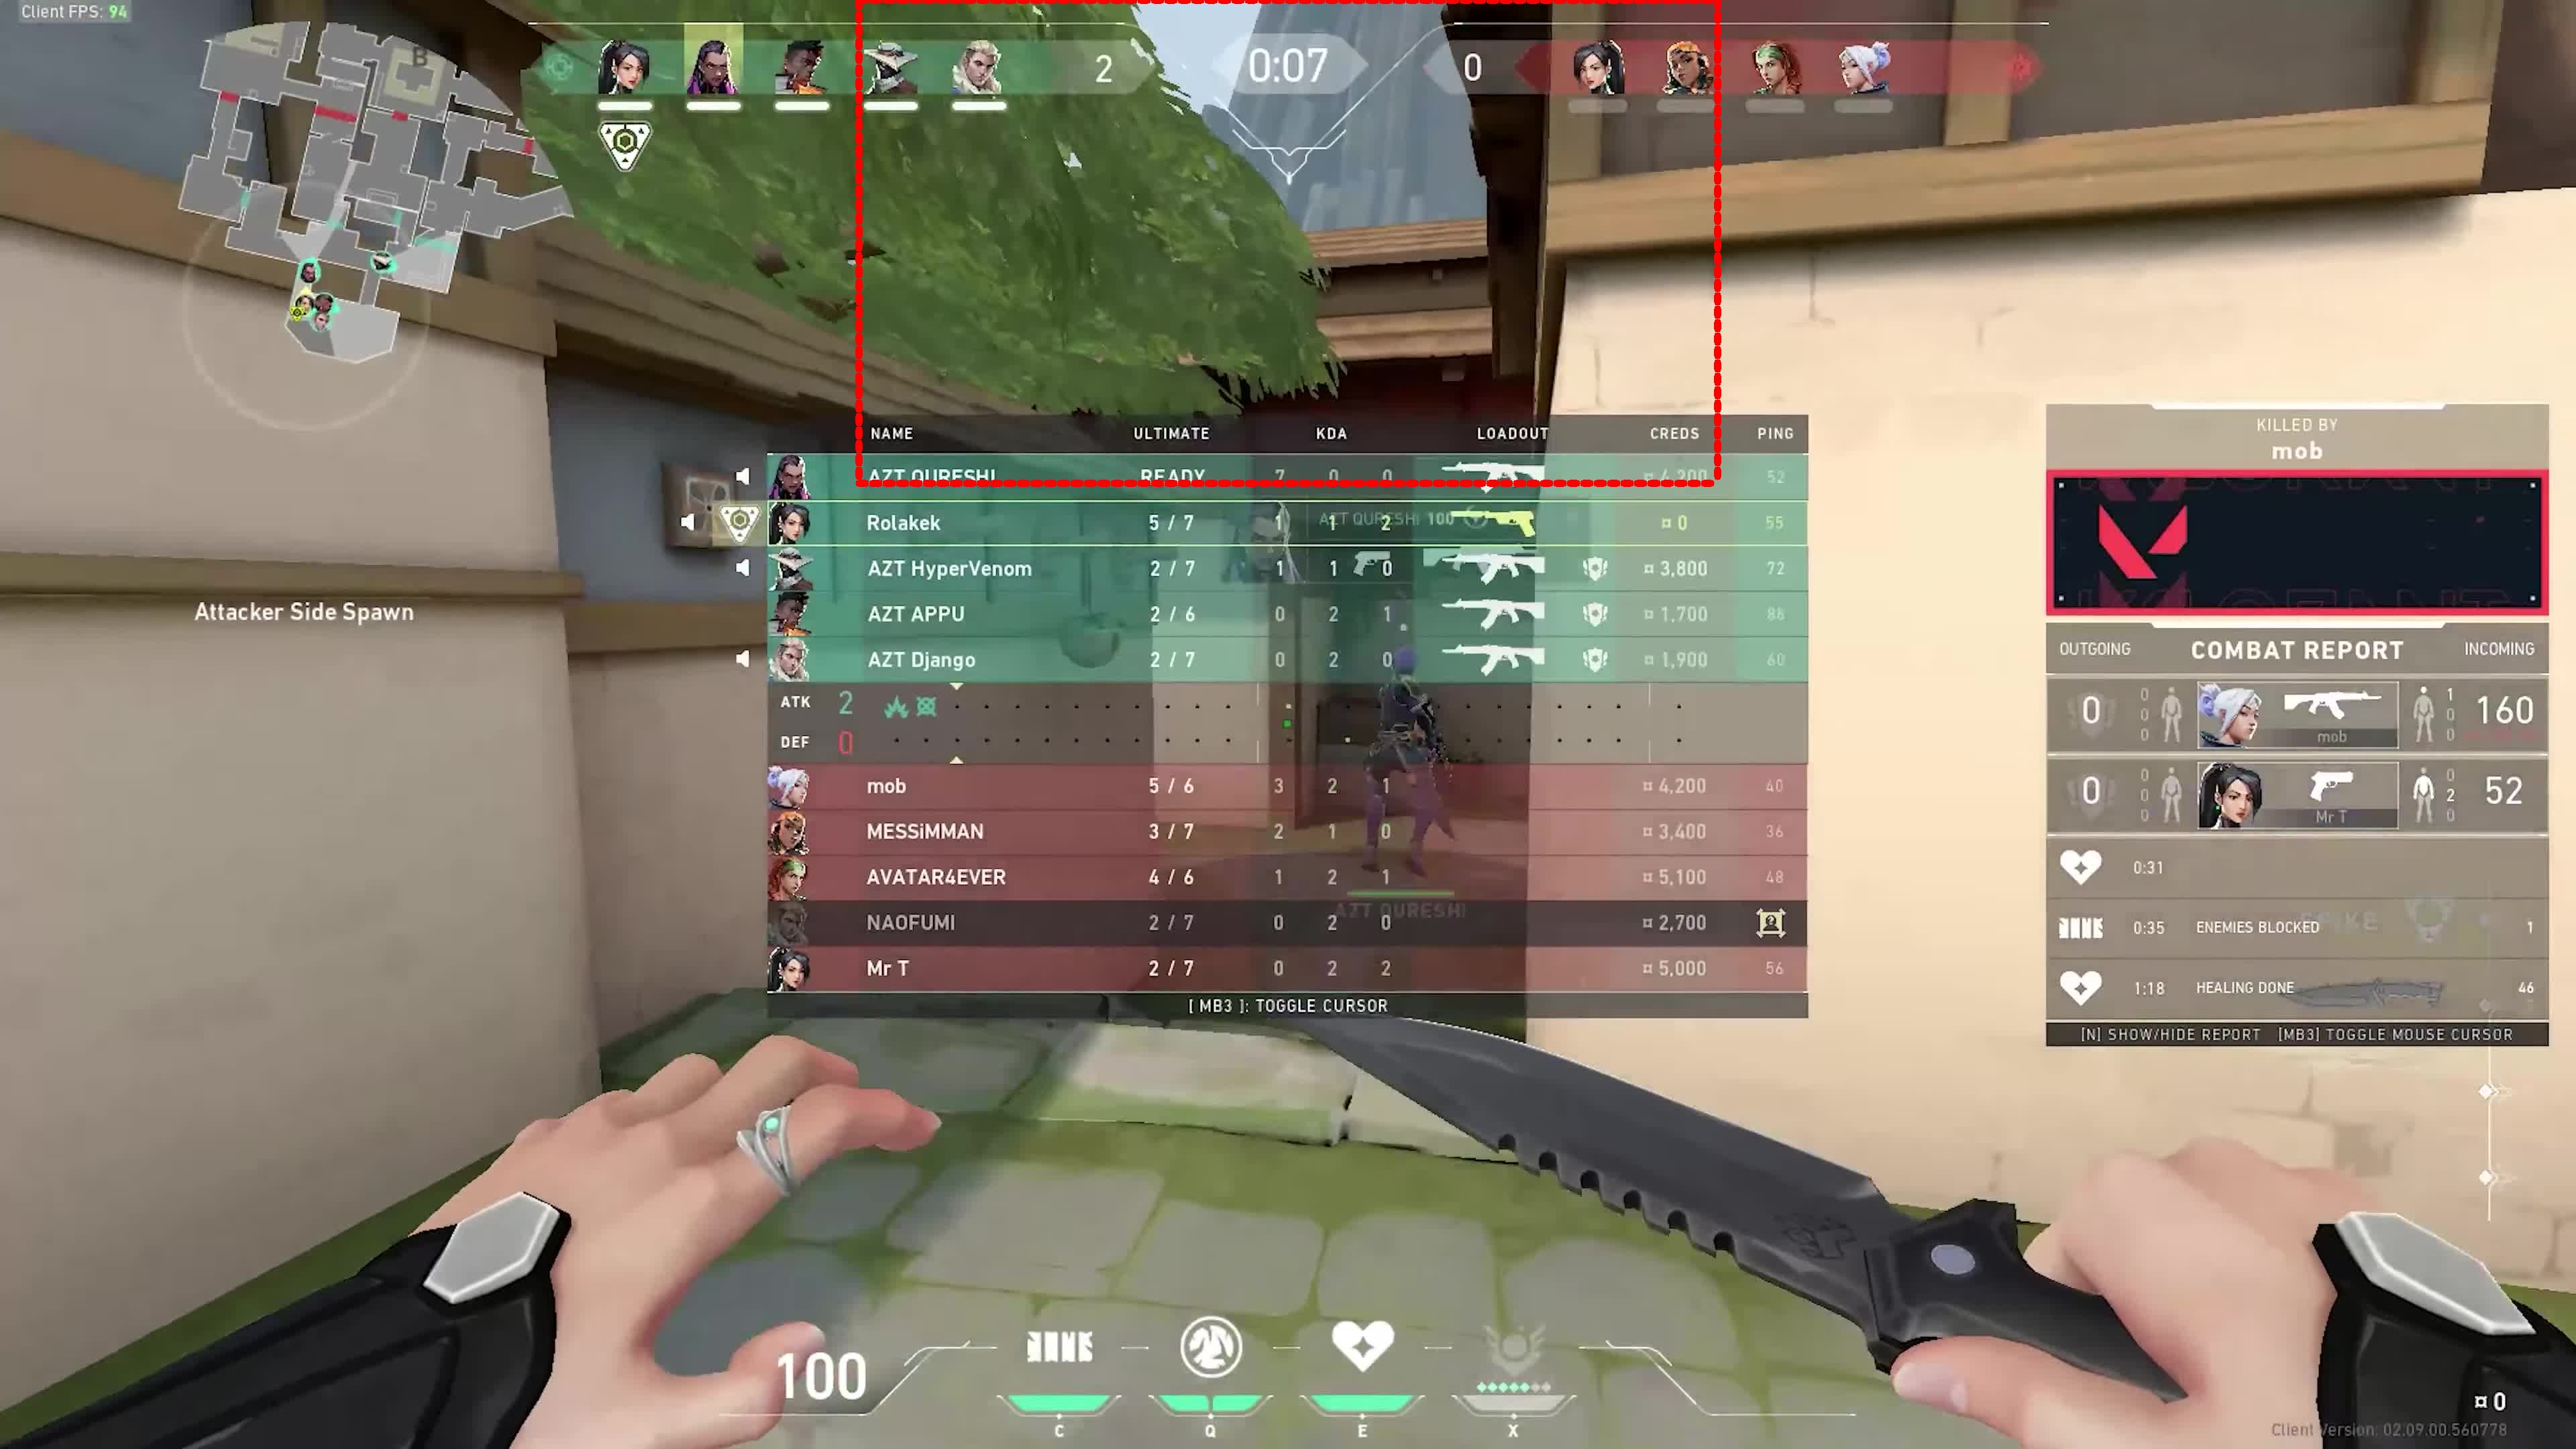
\includegraphics[width=\textwidth]{ressources/roi.jpg}
    \caption{Example of a cropped region of interest from a gaming frame.}
    \label{fig:roi_example}
\end{figure}
This newly selected area will serve as our background for the rest of the synthesis process. Then, we select an icon from our set of templates, which will be our target during training. We overlay our icon onto the background at the center, and we ensure that the icon is fully contained within the background region by downscaling it slightly and continuously till it fits perfectly.
\begin{figure}[H]
    \centering
    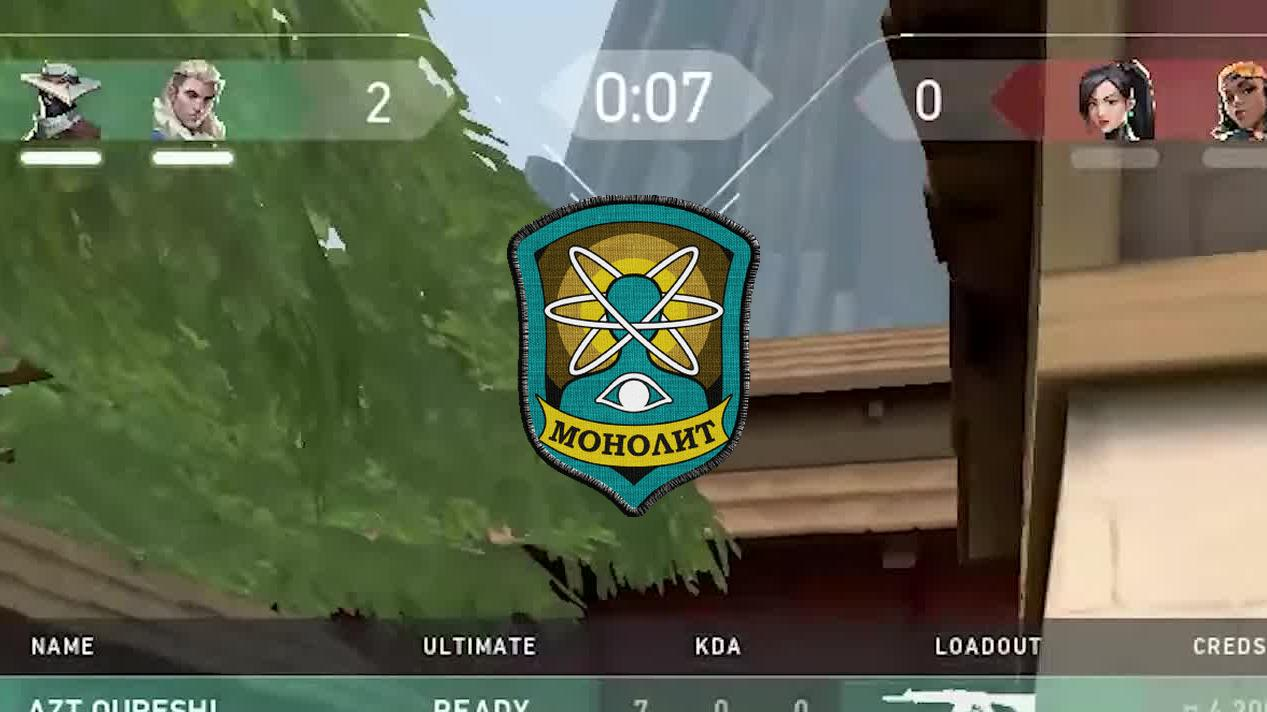
\includegraphics[width=0.9\textwidth]{ressources/image1.jpg}
    \caption{Example of the icon overlaid on the background.}
    \label{fig:overlay_example}
\end{figure}
While this describes our general design principle for synthetic data generation, the process was refined over several iterations to address specific challenges such as background complexity, icon transformations, and the robustness of extracted keypoints.
\begin{comment}
\begin{itemize}
    \item Scaling: We randomly scale the icon by a factor between 1.0 and 3.0
    \item Rotation: We randomly rotate the icon by an angle between -30 and 30 degrees.
    \item Translation: We randomly translate the icon by a few pixels in both x and y
          directions, while insuring that the icon remains within the bounds of the
          background.
    \item Color Jittering: We apply random changes to the brightness, contrast,
          saturation, and hue of the icon to create variations in appearance.
    \item Gaussian Noise: We add random Gaussian noise to the icon to simulate real-world
          noise.
\end{itemize}
\end{comment}

\begin{figure}[H]
    \centering
    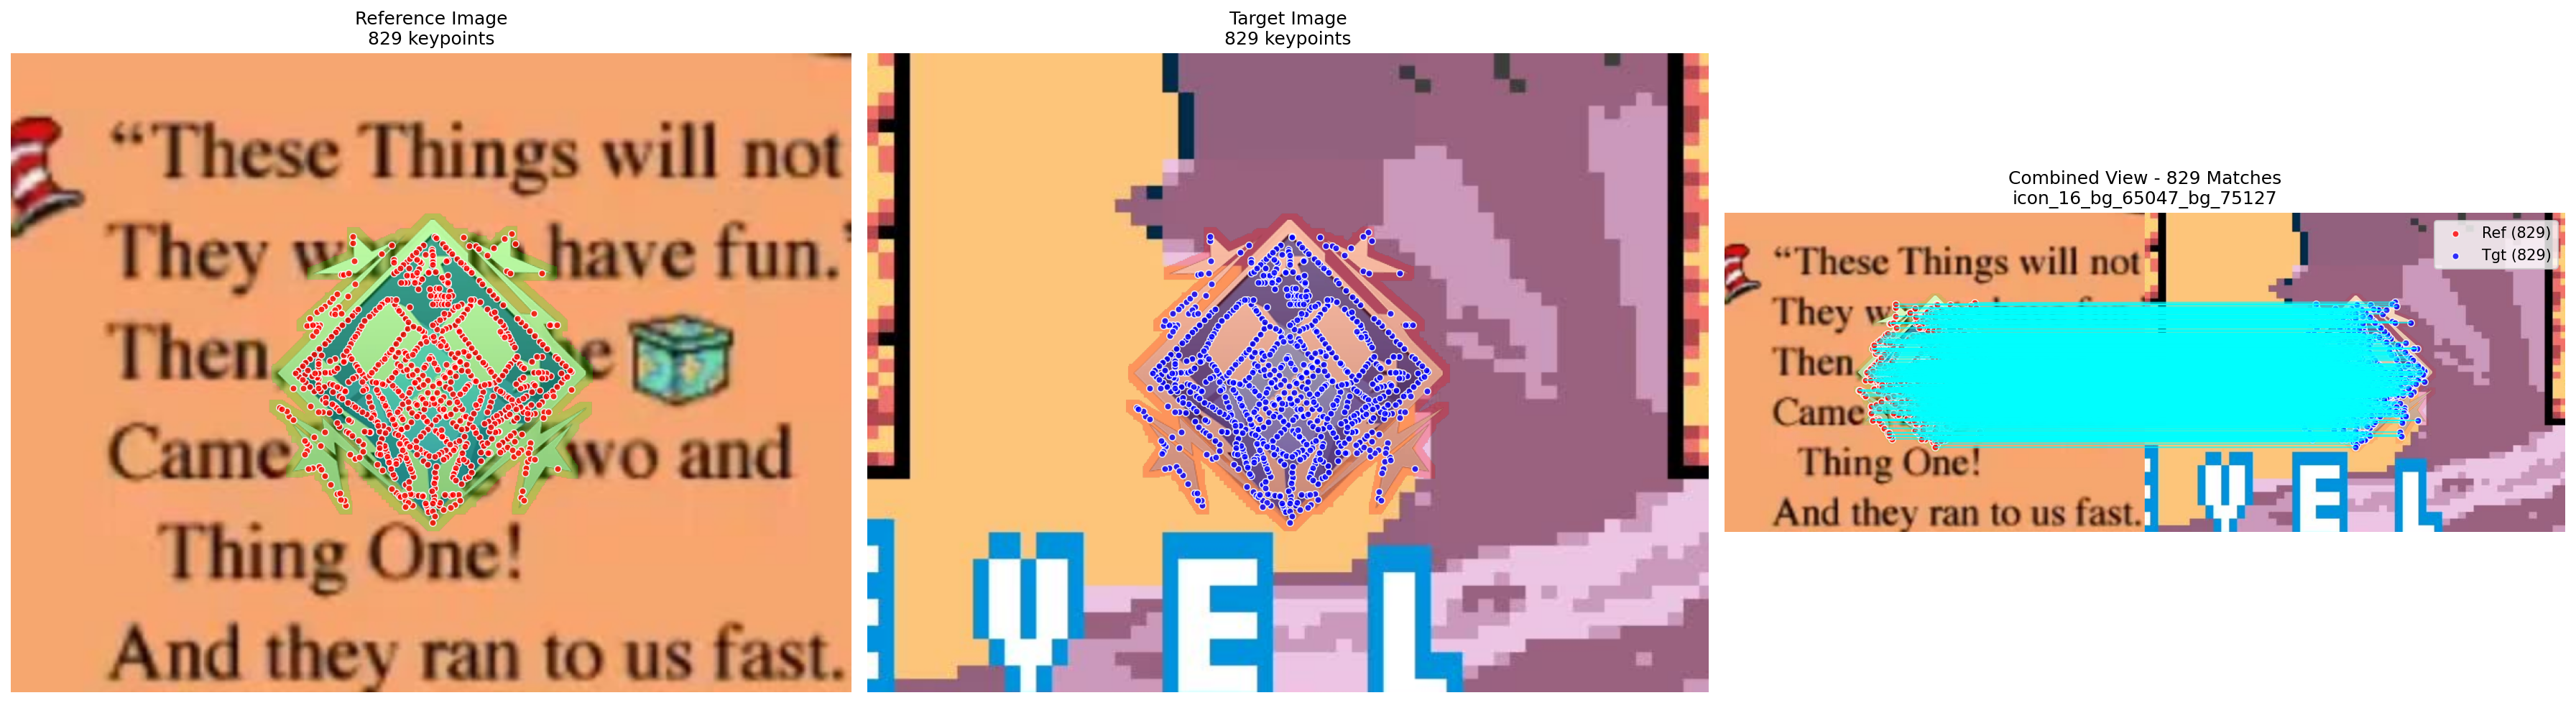
\includegraphics[width=\textwidth]{ressources/example_data1.png}
    \caption{Example of the synthesis process, showing the background and the overlaid icon as well as the detected keypoints and masks.}
    \label{fig:synthesis_example1}
\end{figure}
\begin{figure}[H]
    \centering
    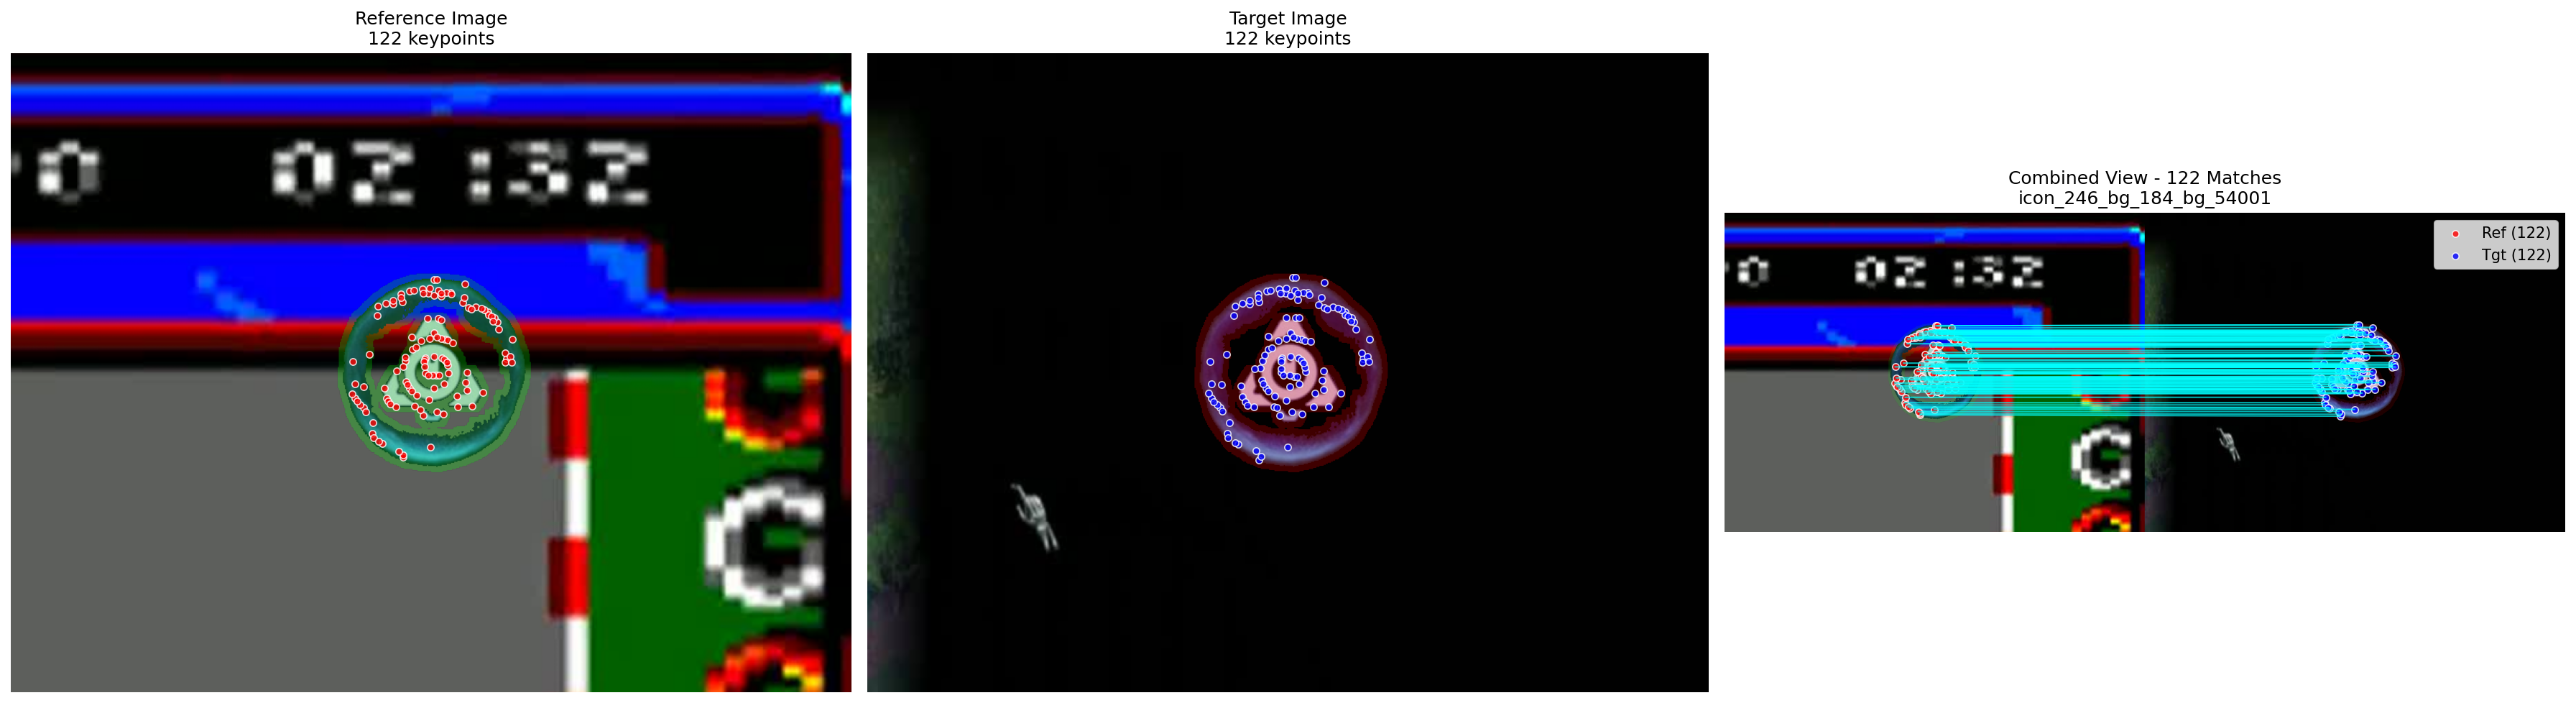
\includegraphics[width=\textwidth]{ressources/example_data2.png}
    \caption{Example of the synthesis process, showing the background and the overlaid icon as well as the detected keypoints and masks.}
    \label{fig:synthesis_example2}
\end{figure}

\section{Training Procedure \& Experimental Setup}
Our chosen approach consists of training the network on synthetic data using a
teacher-student framework. In the early stages, we kept the same teacher model
used by XFeat\cite{xfeat2023}. ALIKE, was used as a third party teacher tool to
extract ground truth keypoints from our training images.
\begin{figure}[H]
    \centering
    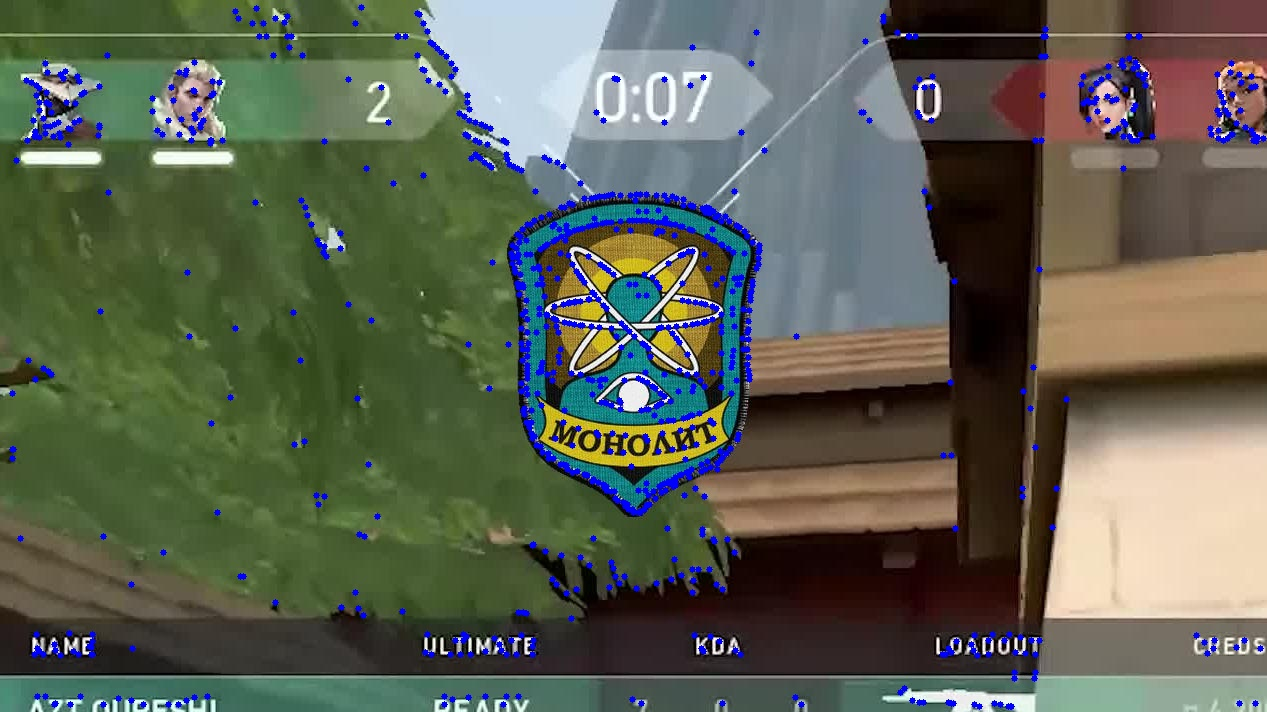
\includegraphics[width=0.8\textwidth]{ressources/image1_keypoints.jpg}
    \caption{Overview of extraction process.}
    \label{fig:teacher_student}
\end{figure}
We then generate a binary mask showing the presence of the icon within the background.
\begin{figure}[H]
    \centering
    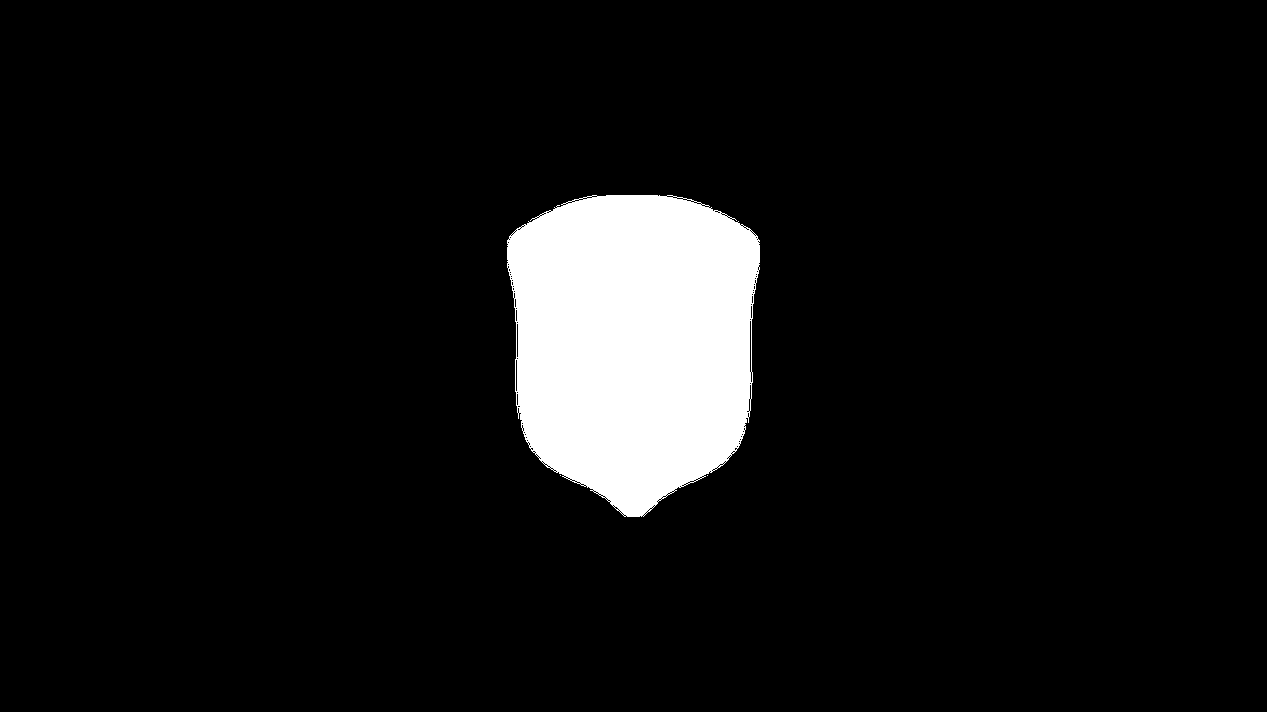
\includegraphics[width=0.8\textwidth]{ressources/mask_1.png}
    \caption{Example of the binary mask generated for the icon.}
    \label{fig:binary_mask}
\end{figure}
This mask is used to filter out keypoints that do not belong to the icon, ensuring that only relevant features are considered during training. This would teach the model to focus only the keypoints and data existing within the icon region , which is what we want to achieve.
\begin{figure}[H]
    \centering
    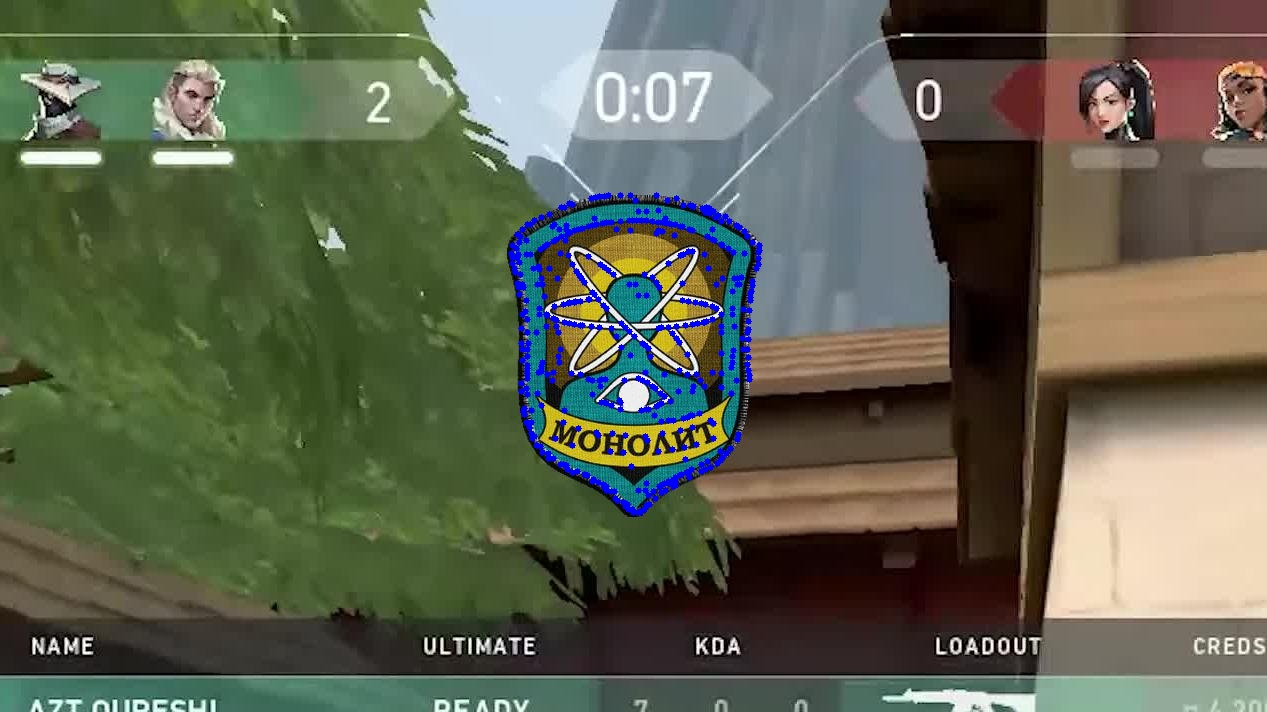
\includegraphics[width=0.8\textwidth]{ressources/image1_keypoints_masked.jpg}
    \caption{Overview of filtering process.}
    \label{fig:teacher_student}
\end{figure}
\section{Quantitative Results}
\section{Qualitative Results}
\section{Analysis \& Discussion}
\subsection{Compare results with SIFT, ORB, XFeat}
\subsection{Discuss trade-offs: speed vs. accuracy.}
\subsection{Link back to performance targets from Chapter 4.}
\subsection{Tie to the research gap from Chapter 3.}
